% Specify the type of document
\documentclass[12pt]{article}

% Load a number of useful packages
\usepackage{graphicx}
\usepackage{amsmath,amssymb,amsfonts,amsthm}
\usepackage[margin=1.0in]{geometry}
\usepackage[colorlinks=true]{hyperref}
\usepackage{gensymb}
\usepackage[font=small, labelfont=bf]{caption}
\usepackage{cite}
\usepackage{commath}
\usepackage{multicol}
\usepackage[utf8]{inputenc}
\usepackage{cancel}
\usepackage[english]{babel}
\usepackage{tikz}
\usetikzlibrary{shapes.misc,shadows}
\usepackage{listings}
\usepackage{caption}
\usepackage{changepage}
\usepackage{color, xcolor}
\usepackage[caption=false,font=footnotesize]{subfig}
\usepackage{hyperref}
\usepackage[utf8]{inputenc}
\usepackage[english]{babel}
\usepackage{tikz}
\usetikzlibrary{shapes.misc,shadows}
\usepackage{listings}
\usepackage{color, xcolor} %red, green, blue, yellow, cyan, magenta, black, white
\definecolor{mygreen}{RGB}{28,172,0} % color values Red, Green, Blue
\definecolor{mylilas}{RGB}{170,55,241}
\definecolor{red}{RGB}{255,0,0}
\hypersetup{
    colorlinks=true,
    linkcolor=blue,
    filecolor=magenta,
    urlcolor=orange,
}

% Two more packages that make it easy to show MATLAB code
\usepackage[T1]{fontenc}
\usepackage[framed,numbered]{matlab-prettifier}
\lstset{
	style = Matlab-editor,
	basicstyle=\mlttfamily\small,
}

% Say where pictures (if any) will be placed
\graphicspath{{./pictures/}}

% Define title, author, and date
\title{AE353: Design Problem 02}
\author{Robotic Controllability}
\date{March 8, 2019}

% Start of document
\begin{document}

% Put the title, author, and date at top of first page
\maketitle


\begin{section}{Goal}
The code, \lstinline!DesignProblem02! simulates a ``gravity-assisted underactuated robot arm.'' This robot arm has two joints: one controlled, one free.  Optical encoders measure joint angles ($q$) and velocities ($v$).  The goal is to make the second joint angle track a piecewise-constant reference trajectory.

\label{req}
\label{sec:1.1} \subsection{Requirements}
A \textit{requirement} is a property that the system must have in order to solve the problem.
\begin{adjustwidth}{20pt}{0pt}
    {\em The second joint angle, $q_2$ shall follow the piece-wise function henceforth defined as \emph{$\alpha$}  and have an accuracy of $\pm 2\degree$ with convergence within $3$ seconds.}
\end{adjustwidth}
\label{alpha}
\begin{equation}
    \alpha_i =
    \begin{cases}
        q_2 = 5\degree & t \leq 5 \\
        q_2 = 10\degree & 5 < t \leq 10 \\
        q_2 = 15\degree & 10 < t \leq 15 \\
        q_2 = 0\degree & 15 < t
    \end{cases}
\end{equation}

\subsection{Verification}
A \textit{verification} is a test that is performed to verify the system meets the requirements set in section (\textcolor{red}{1.1}).
\begin{adjustwidth}{20pt}{0pt}
    \lstinline{DesignProblem02('Controller', 'datafile', 'data.mat')} will run and the data points from \lstinline{'data.mat'} will calculate the error between the second joint angle, $q_2$, and reference value, $\alpha$, at each time-step value of $\Delta t = 0.25 [s]$ by the following computation:
    \[
    E(t) = |q_2(t) - \hyperref[alpha]{\alpha}|
    \] If $E \leq 2\degree$ with an accuracy of over 70\%, then the requirement is satisfied.
\end{adjustwidth}
\end{section}

\newpage

\begin{section}{State Space Model}
The motion of the robot is governed by ordinary differential equations with the form
\begin{equation}
\label{eqEOM}
M(q) \ddot{q} + C(q,\dot{q})\dot{q} + N(q,\dot{q}) = \tau \mbox{ where},
\end{equation}
\begin{equation*}
q = \begin{bmatrix} q_{1} \\ q_{2} \end{bmatrix}, 
\dot{q} = \begin{bmatrix} v_{1} \\ v_{2} \end{bmatrix},
\tau = \begin{bmatrix} \tau_{1} \\ 0 \end{bmatrix}
\end{equation*}
$q$ is a matrix of joint angles, $\dot{q}$ is a matrix of joint velocities, $\tau$ is a matrix of applied torques, and $M(q), C(q,\dot{q}), N(q,\dot{q})$, are matrix-valued functions of $q$ and/or $\dot{q}$. These functions depend on a number of parameters.  Before linearizing, it is important to solve for $\ddot{q}$:
\begin{equation}
    \ddot{q} = \frac{\tau - C(q,\dot{q})\dot{q} - N(q, \dot{q})}{M(q)}
\end{equation}
\subsection{Linearization}
Now the \lstinline{Jacobian()} of $\ddot{q}$ and $\dot{q}$ will be utilized for $A$ and $\frac{\tau}{M(q)}$ to find $B$ (for detailed code on calculation of pertinent linearization values, please refer to this [\href{https://drive.google.com/file/d/1SKI_ZmOP5XFAXiwL9oEj5oYMP6tqxz1v/view?usp=sharing}{\textbf{script}}]):
\[
     \textbf{A} = [\ddot{q}]_{(\dot{q})} = 
     \begin{bmatrix}
         0 & 0 & 1 & 0 \\
         0 & 0 & 0 & 1 \\
         5.5465 & -61.2335 & -1.5762 & -0.8327 \\
         -1.9024 & -10.7824 & -0.2776 & -0.3690
     \end{bmatrix}, \enspace
     \textbf{B} =
     \begin{bmatrix}
         0 \\ 0 \\ 3.1525 \\ 0.5551
     \end{bmatrix}
\]
\[
    u = -K\cdot x
\]

\subsection{Controllability}
The $Q$ matrix was a scaled \lstinline{5*eye(size(A))} matrix and $R$ was selected to enable the controller to meet the goals in a precise quantity of time.  With these values, the controller may now be designed and implemented for the \emph{State Space Model}.  To confirm controllability, the following test will be implemented on the linearized system: \lstinline{rank(W)} $= 4$ in \lstinline{FindingValues.m}.

\label{sec:2.3} \subsection{Reference Tracking}
In order to enable reference tracking, a component must be added the input:
\[ u = -K\cdot x + \mathbf{k_{ref}\cdot r}, \mbox{ for } k_{ref} = \lstinline{inv(-C*inv(A-B*K)*B)} \mbox{ and } K = \lstinline{lqr(A,B,Q,R)} \]

\subsection{Disturbance Rejection}
If disturbance is introduced to the simulation, Integral action may be utilized to oppose the effects of unknown disturbance.
\[ u = -K\cdot x + k_{ref}\cdot r + d - \mathbf{k_{int}\cdot v} \mbox{ for } v = \int_0^t (q_2(\tau) - r(\tau)) d\tau\]

\end{section}

\begin{section}{Control Design}
The goal, as stated in \hyperref[req]{requirements}, is to make the arm converge asymptotically, tracing points at $q_2 = \hyperref[alpha]{\alpha}$ every 5 seconds and reach convergence within 3 seconds.  In order to implement this, the $A,B,C,D$ values must be structured in the following State Space model:
\[
    \dot{x} = Ax + Bu , \enspace
    y = Cx + Du, \enspace \\
    u = -Kx + k_{ref}r + d - k_{int} v
\]
with
\[
    x =
    \begin{bmatrix}
        q_1 \\ q_2 \\ v_1 \\ v_2
    \end{bmatrix}
\]
The controller will be implemented by designating the values for $r$, $K$, and $k_{ref}$ in order to track and pursue the desired $q_2$ angle at the desired time, mitigate the settling time, and optimize the efficiency respectively.  In section (\hyperref[sec:2.3]{2.3}), the \emph{\textbf{L}inear \textbf{Q}uadratic \textbf{R}egulator} function was utilized to find the optimal value for $K$.  This will enable the controller to reach the desired joint angles in the least amount of time/cost.  Two trials will be run, one without disturbance and one accounting for some unknown disturbance.  In the codes, colleagues are provided the option to select \emph{1} or \emph{2}:
\begin{itemize}
    \item $1$ utilizes \lstinline{Controller1.m}, a controller which does not include Integral Action.
    \item $2$ utilizes \lstinline{Controller2.m}, a controller which attempts to use Integral Action.
\end{itemize}
\textbf{Figure 1.}$_{(Undisturbed)}$ and \textbf{Figure 2.}$_{(Disturbed)}$ display the results of implementing the controller on the swinging arm simulation.

\centering
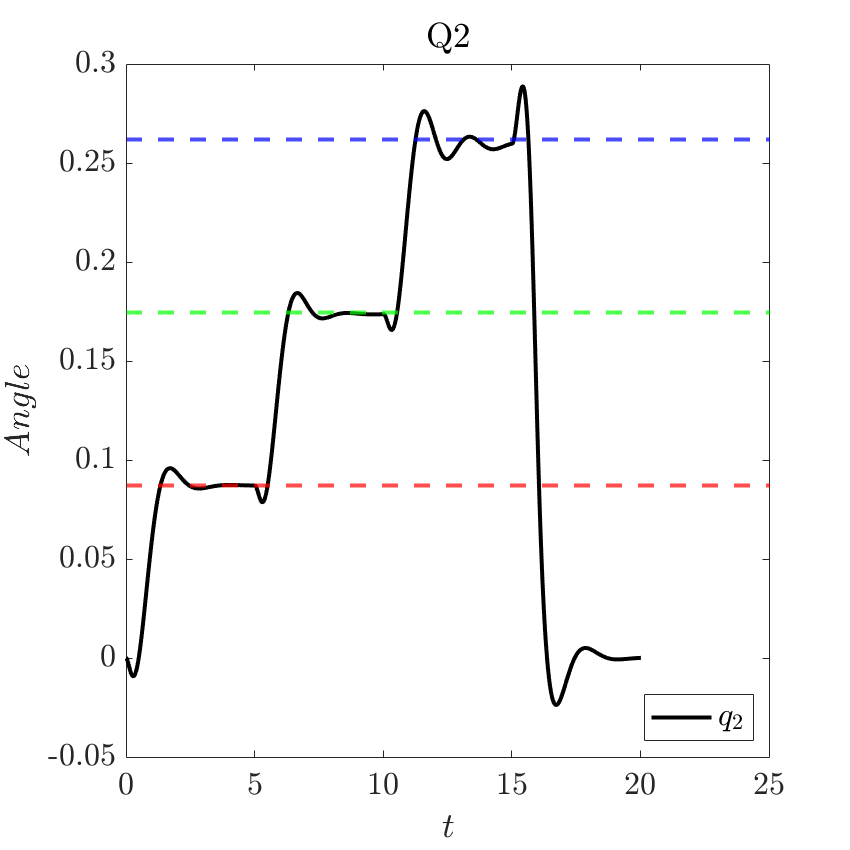
\includegraphics[scale=0.60]{q2_vs_t_no_disturb.png}
\captionof{figure}{}
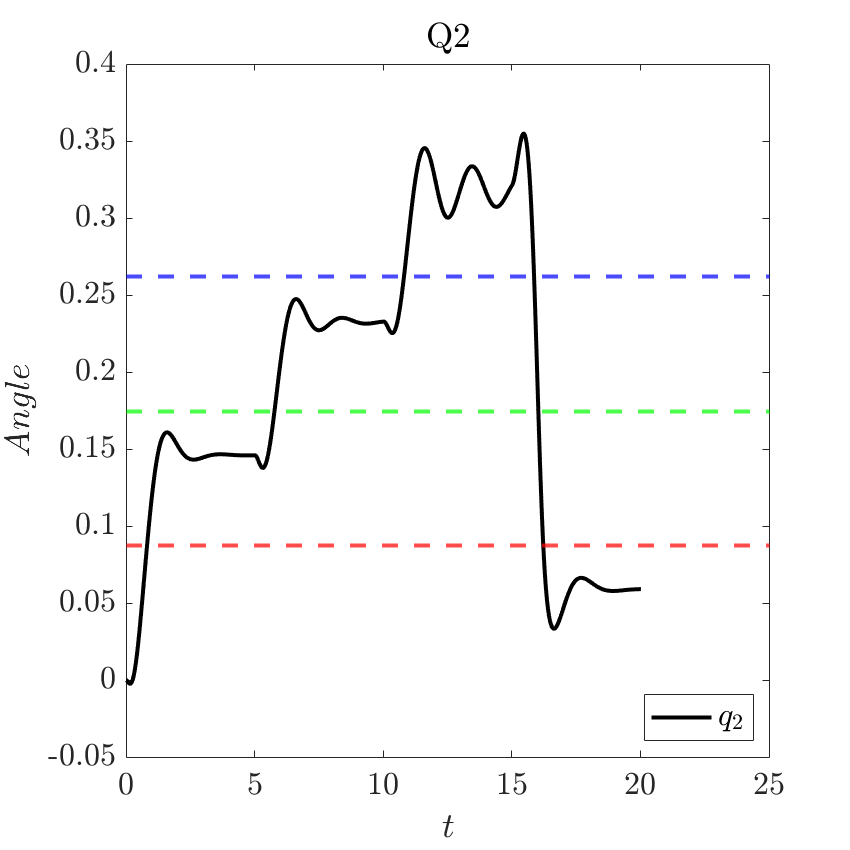
\includegraphics[scale=0.60]{q2_vs_t_disturb.png}
\captionof{figure}{}
\end{section}

\begin{section}{Conclusions}
This simulation observes one rotational motor and one free joint on a "gravity-assisted under-actuated robot arm."  The requirements for this controller test were defined as such from section (\hyperref[sec:1.1]{1.1}):  \emph{The second joint angle, $q_2$ shall follow the piece-wise function as defined as \hyperref[alpha]{$\alpha$} and maintain an accuracy of $\pm 2\degree$ and converge within 5 seconds.}  To test this requirement, a verification was implemented in the \lstinline{Test.m} script which observed the absolute value of the difference between $q_2(t)$ and $\alpha$.  If the error term is of the accuracy of $70\%$ or greater, the controller would be declared successful in this requirement.  After linearizing the system, various tests were conducted, utilizing \lstinline{eig(A)} and \lstinline{rank(W)} to determine asymptotic stability of the open system and controllability.  It was interesting to realize that the system was not truly asymptotically stable independently, but maintained controllability.  Two trials were conducted, one involving no disturbance and the other simulating some unknown disturbance.  In order to attempt to compensate for said disturbance, integral action was utilized in the input, i.e. $u = -Kx + k_{ref}r + d - k_{int}v$ for $v = \int_0^t(q_2{\tau} - r(\tau)) d\tau$.  After selecting the desired controller setup in the \lstinline{Test.m} file, graphs such as those shown as \textbf{Figure 1.} and \textbf{Figure 2.} were produced.  For the case of no disturbance, the controller changed the second joint angle according to $\alpha$ with a settling time of roughly $2$ seconds and maintained accuracy of within $0.1 \degree$; the verification portion of the script returned an accuracy of approximately $79.7\%$ and $\therefore$ passed the verification process.  The disturbance trial, on the other hand, did not have much success and repeatedly contained more than $80\%$ error, indicating the derivation for $v$ was not properly functional.  Ultimately, the requirements were satisfied by test of the verification for the undisturbed trial by utilizing optimized state space model, $u = -Kx$, and reference tracking for a piece-wise, $\alpha$, function, $u = -k_{ref}r$.


\end{section}






% End of document (everything after this is ignored)


\end{document}